%%%%%%%%%%%%%%%%%%%%%%%%%%%%%%%%%%%%%%%%%
% Thin Sectioned Essay
% LaTeX Template
% Version 1.0 (3/8/13)
%
% This template has been downloaded from:
% http://www.LaTeXTemplates.com
%
% Original Author:
% Nicolas Diaz (nsdiaz@uc.cl) with extensive modifications by:
% Vel (vel@latextemplates.com)
%
% License:
% CC BY-NC-SA 3.0 (http://creativecommons.org/licenses/by-nc-sa/3.0/)
%
%%%%%%%%%%%%%%%%%%%%%%%%%%%%%%%%%%%%%%%%%

%----------------------------------------------------------------------------------------
%	PACKAGES AND OTHER DOCUMENT CONFIGURATIONS
%----------------------------------------------------------------------------------------

\documentclass[a4paper, 11pt]{article} % Font size (can be 10pt, 11pt or 12pt) and paper size (remove a4paper for US letter paper)

\usepackage[protrusion=true,expansion=true]{microtype} % Better typography
\usepackage{graphicx} % Required for including pictures
\usepackage{wrapfig} % Allows in-line images
\usepackage[section]{placeins} % Prevent images float to other sec
\usepackage{mathpazo} % Use the Palatino font
\usepackage[T1]{fontenc} % Required for accented characters
\linespread{1.05} % Change line spacing here, Palatino benefits from a slight increase by default
\usepackage[export]{adjustbox}
\usepackage{cite} % to place citations in the right order

% Use placeins with subsections
\makeatletter
\AtBeginDocument{%
  \expandafter\renewcommand\expandafter\subsection\expandafter{%
    \expandafter\@fb@secFB\subsection
  }%
}
\makeatother

\makeatletter
\renewcommand\@biblabel[1]{\textbf{#1.}} % Change the square brackets for each bibliography item from '[1]' to '1.'
\renewcommand{\@listI}{\itemsep=0pt} % Reduce the space between items in the itemize and enumerate environments and the bibliography

\renewcommand{\maketitle}{ % Customize the title - do not edit title and author name here, see the TITLE block below
\begin{flushright} % Right align
{\LARGE\@title} % Increase the font size of the title

\vspace{50pt} % Some vertical space between the title and author name

{\large\@author} % Author name
\\\@date % Date

\vspace{40pt} % Some vertical space between the author block and abstract
\end{flushright}
}

%----------------------------------------------------------------------------------------
%	TITLE
%----------------------------------------------------------------------------------------

\title{\textbf{Studying three-dimensional genome organization using Hi-C}} % Title
%Evaluation of state-of-the-art methods} % Subtitle
\author{\textsc{Harris A. Lazaris}\\ % Author
{\textit{BMI Final Project}}} % Course

\date{\today} % Date

%----------------------------------------------------------------------------------------

\begin{document}

\maketitle % Print the title section

%----------------------------------------------------------------------------------------
%	ABSTRACT AND KEYWORDS
%----------------------------------------------------------------------------------------

\renewcommand{\abstractname}{Summary} % Uncomment to change the name of the abstract to something else

\begin{abstract}

\end{abstract}

\hspace*{3,6mm}\textit{Keywords:} Hi--C, 3D genome organization, evaluation  % Keywords

\vspace{30pt} % Some vertical space between the abstract and first section

%----------------------------------------------------------------------------------------
%	ESSAY BODY
%----------------------------------------------------------------------------------------

\section*{Introduction}

\subsection*{Background information}

The three-dimensional (3D) organization of the human genome and its relationship with genome function, remain largely unexplored. In the last 15 years however, various techniques have been developed that promise to shed light on this great scientific problem~\cite{Dekker:2013hib}. All these techniques are derivatives of the original chromosome conformation capture (3C) method~\cite{Dekker:2002ib}. A 3C variant is Hi--C~\cite{LiebermanAiden:2009jz}. Hi--C generates an all-by-all genome-wide interaction map~\cite{LiebermanAiden:2009jz,Dekker:2013hib}. As it is shown in Figure~\ref{fig:HiC}, chromatin is cross-linked with formaldehyde and loci that are in close proximity (100-300nm apart in space), are linked covalently. Then, chromatin is fragmented and ligation 
results in hybrid DNA fragments that consist of interacting loci. These fragments are biotin-labeled and then purified (with streptavidin beads), amplified and subjected to next-generation sequencing~\cite{LiebermanAiden:2009jz,Belton:2012eva}.  Different methods have been introduced to improve the accuracy and speed of Hi--C data analysis. An iterative correction method involving machine learning~\cite{Imakaev:2012io} and a second one based on Poisson regression~\cite{Hu:2012es} are two of the most popular ones used for Hi--C data filtering and correction. 

% The Hi-C method
\begin{figure}[!htb]
	\begin{center}
		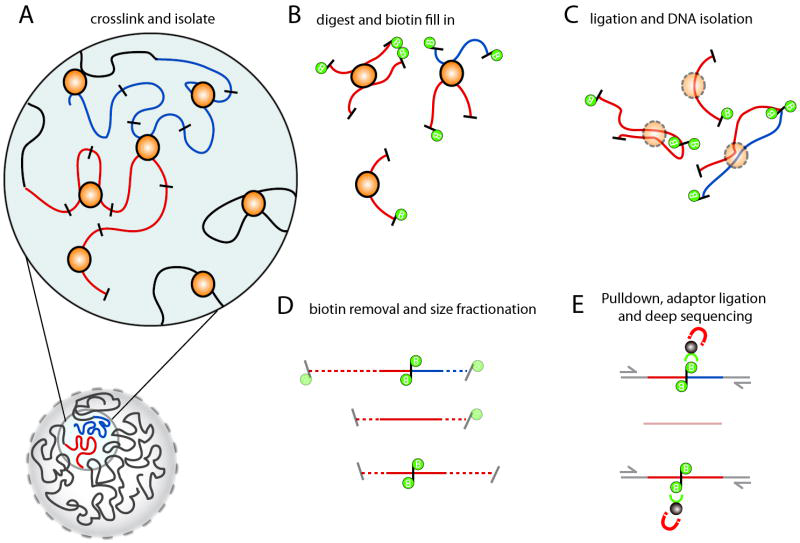
\includegraphics[max size={\textwidth}{\textheight}]{./Figures/Hi-C.pdf}
	\end{center}
	\caption{ An overview of the Hi-C technique. Adapted from Belton, J.M. et al. Methods 58, 268--276 (2012).}
	\label{fig:HiC}
\end{figure}


\subsection*{Motivation}

Studying the three-dimensional organization of the genome is of particular importance as it may offer answer to fundamental questions such as the ones listed below (to mention a few):

\begin{itemize}
\item How chromosomes are organized?
\item Where active genes are located?
\item Is there a tendency for co-regulated genes to co-localize in the nucleus?
\item How important and how frequent ~\emph{cis} and ~\emph{trans} genomic
interactions are for gene transcription?
\end{itemize}

The rationale behind this work is that I would like to evaluate
Hi--C data analysis techniques that are available today --here only HiC
Norm is presented-- and find how they perform in terms of consistency
as well as accuracy. If the existing analysis techniques do not
produce reproducible results, are not effective in terms of resource
usage or fail to produce biologically relevant results, I will have
the opportunity to start developing a new analysis technique that
outperforms the previous ones. 


%------------------------------------------------

\section*{Materials-Methods}
Original data will be used to create contact Hi--C matrices
with counts of \emph{cis} interactions. Then Python scripts
will be written to calculate the normalized interaction matrices that 
are generated when using different enzymes for the Hi--C experiment
(HindIII and NcoI respectively). The best Hi--C normalization method
will be the one where the HindIII and NcoI matrices generated will
have the highest correlation, as if interactions are valid, experiments
with different enzymes should give similar results. 
Numpy and Pandas will be used to generate
and work with the matrices while matplotlib will be used to generate
the corresponding boxplots summarizing the correlations, as well
the heatmaps showing the \emph{cis} interactions between the different
loci. Git will be used during the whole duration of the project to keep track
of the code written and the changes made to the code. Complexity
analysis will be performed when possible. A database will not be created
during this project.
\label{sec:methods}


%------------------------------------------------


\section*{Results}

\subsection*{Complexity--Timing Analysis}

From the figures shown below, it becomes obvious that
the most time-consuming steps in the case of the script 
that gets a file with the coordinates of the interacting
genomic locations as input, performs the binning (splitting
the genome in chinks) and outputs the corresponding contact 
matrix (the matrix with the interactions), is the process
of reading files and writing to files (I/O).

All the other operations (importing modules, list comprehension etc.) take much less time. The timing was performed using a very
small fraction of the actual input file, in order to save
time (so only the first 10 lines where used). 

\begin{figure}[!htb]
	\begin{center}
		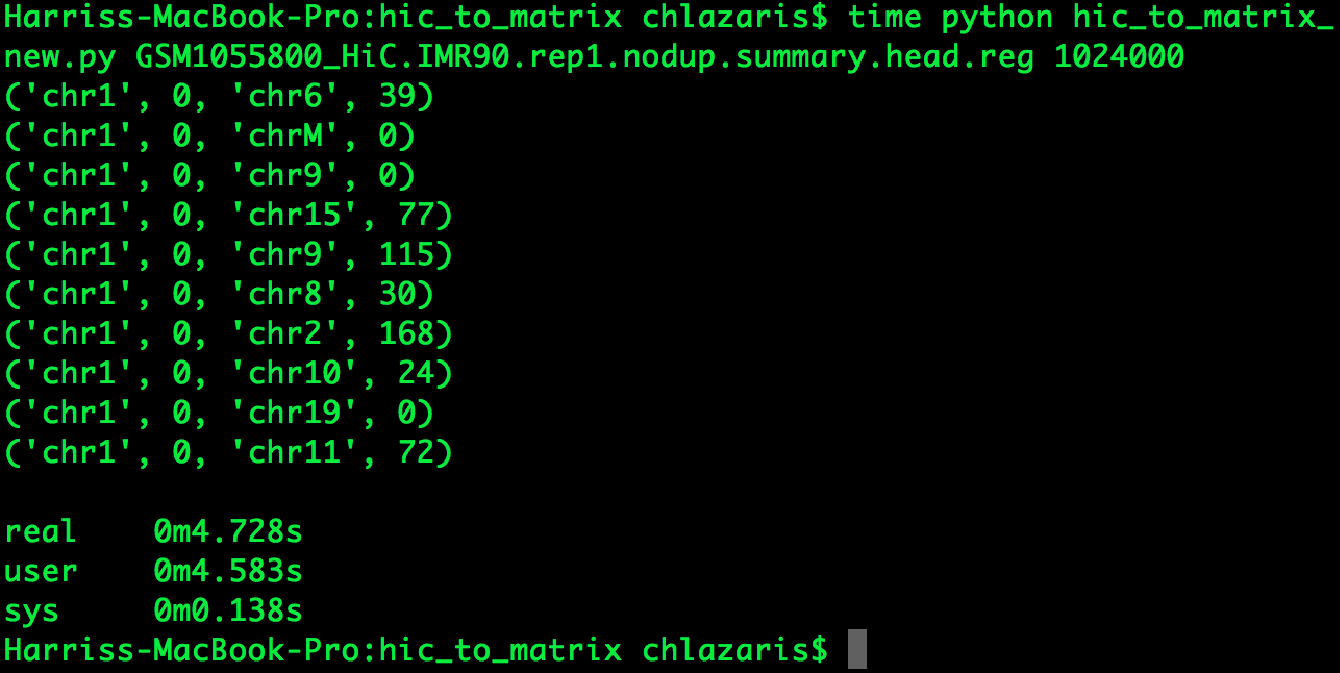
\includegraphics[max size={\textwidth}{\textheight}]{./Figures-Timing/time_whole_script.pdf}
	\end{center}
	\caption{Total time taken by the script to run}
	\label{fig:figure1}
\end{figure}

\begin{figure}[!htb]
	\begin{center}
		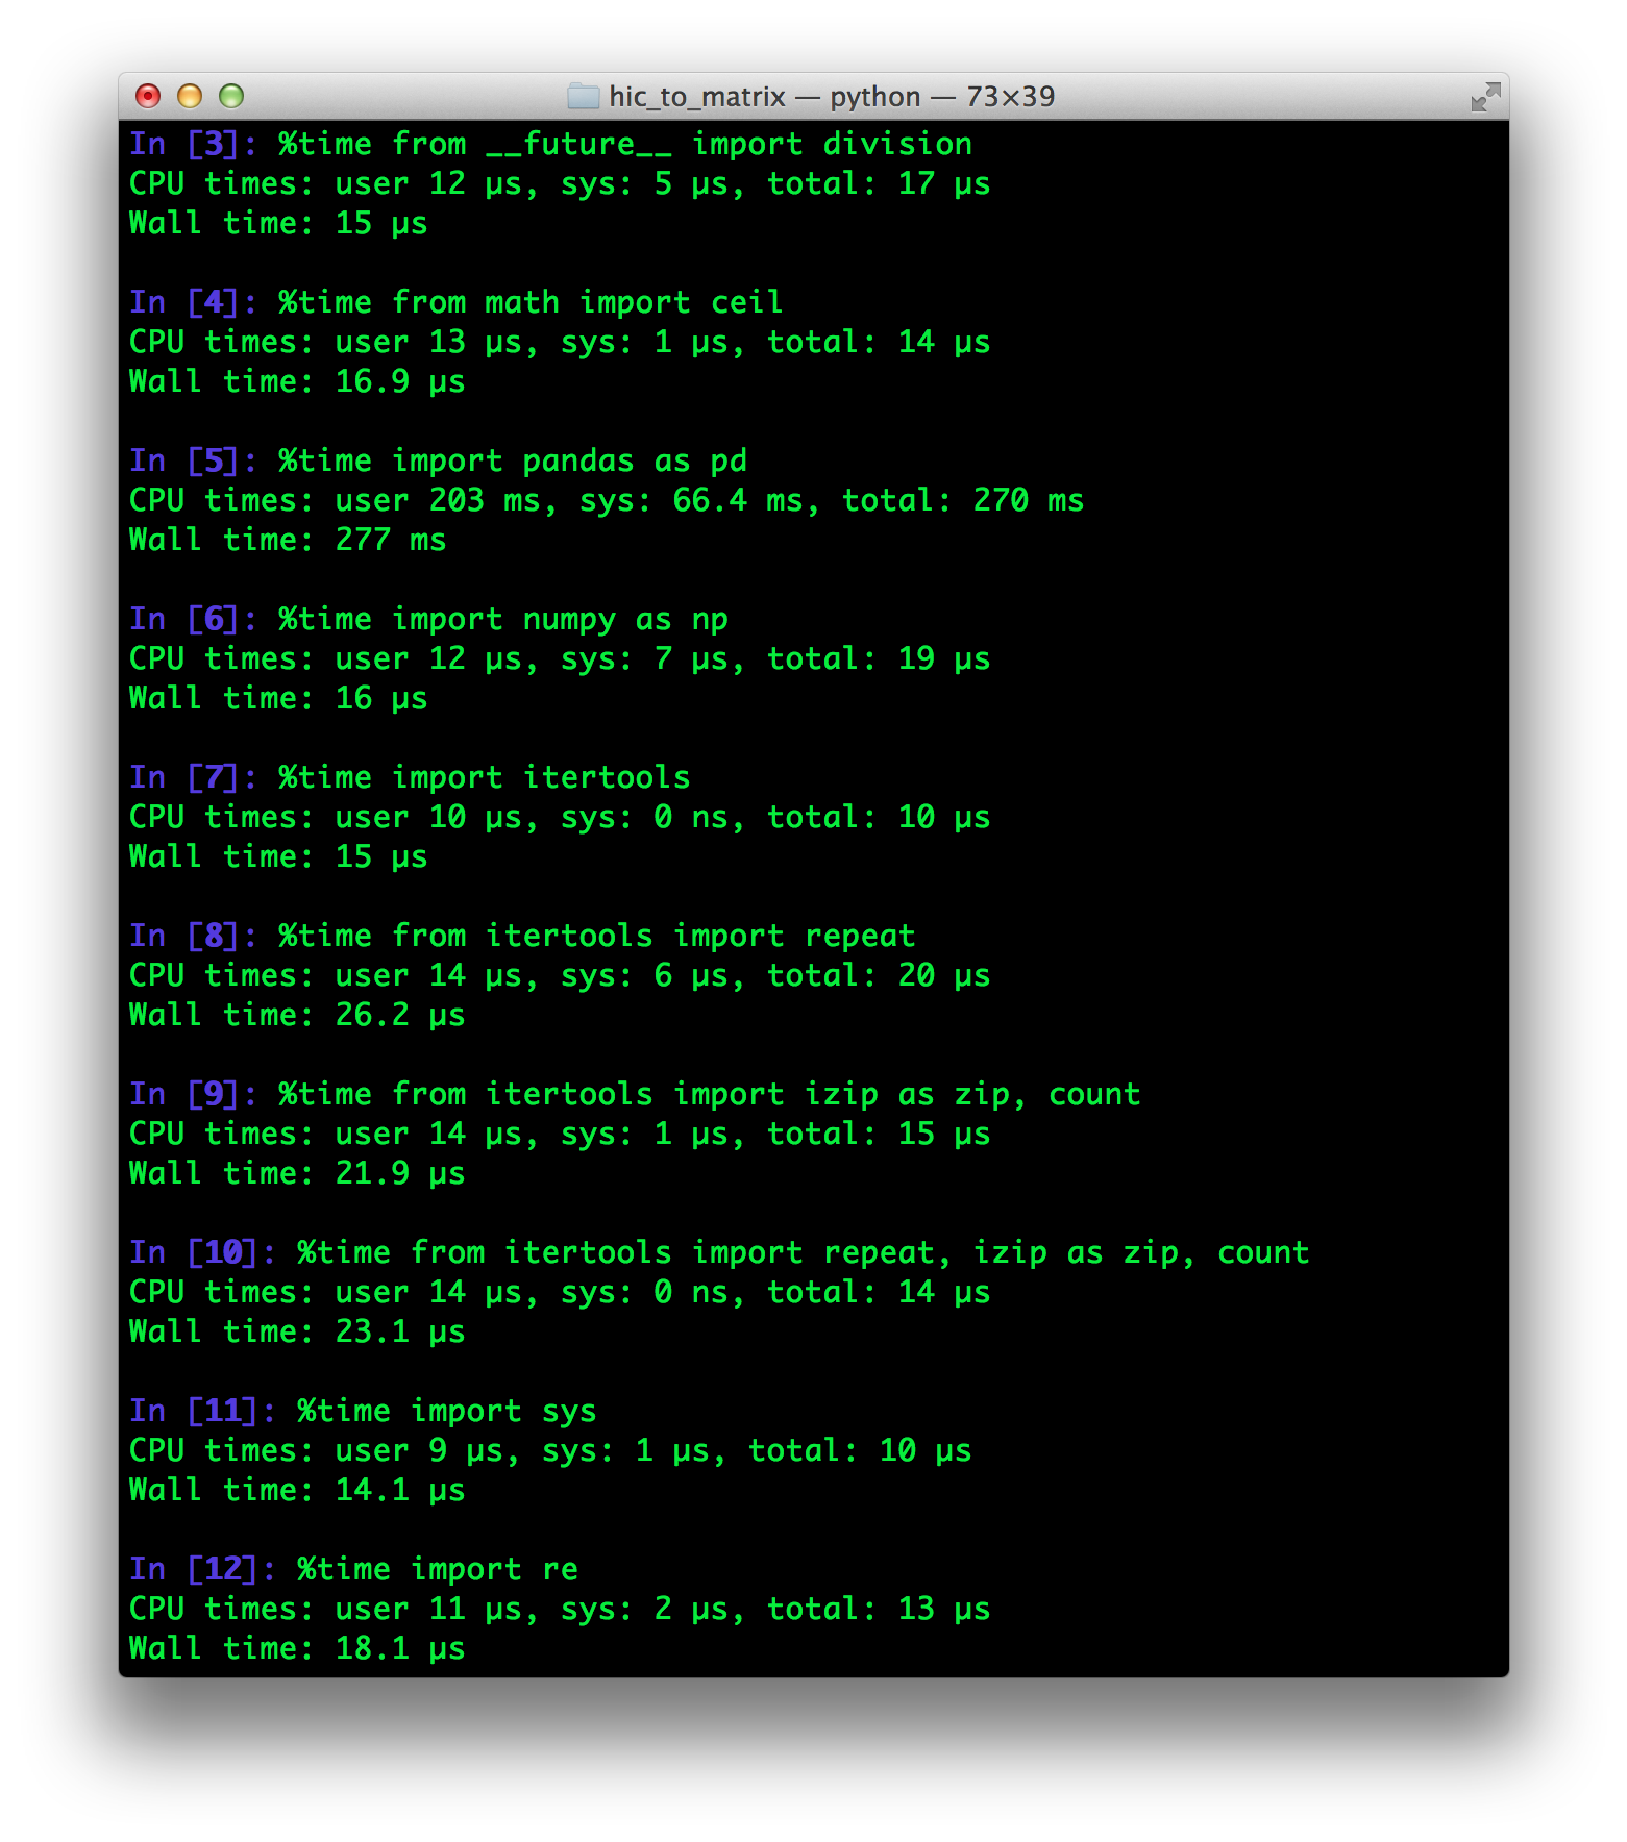
\includegraphics[max size={\textwidth}{\textheight}]{./Figures-Timing/module_import_timing.pdf}
	\end{center}
	\caption{Time taken to import the modules}
	\label{fig:figure2}
\end{figure}

\begin{figure}[!htb]
	\begin{center}
		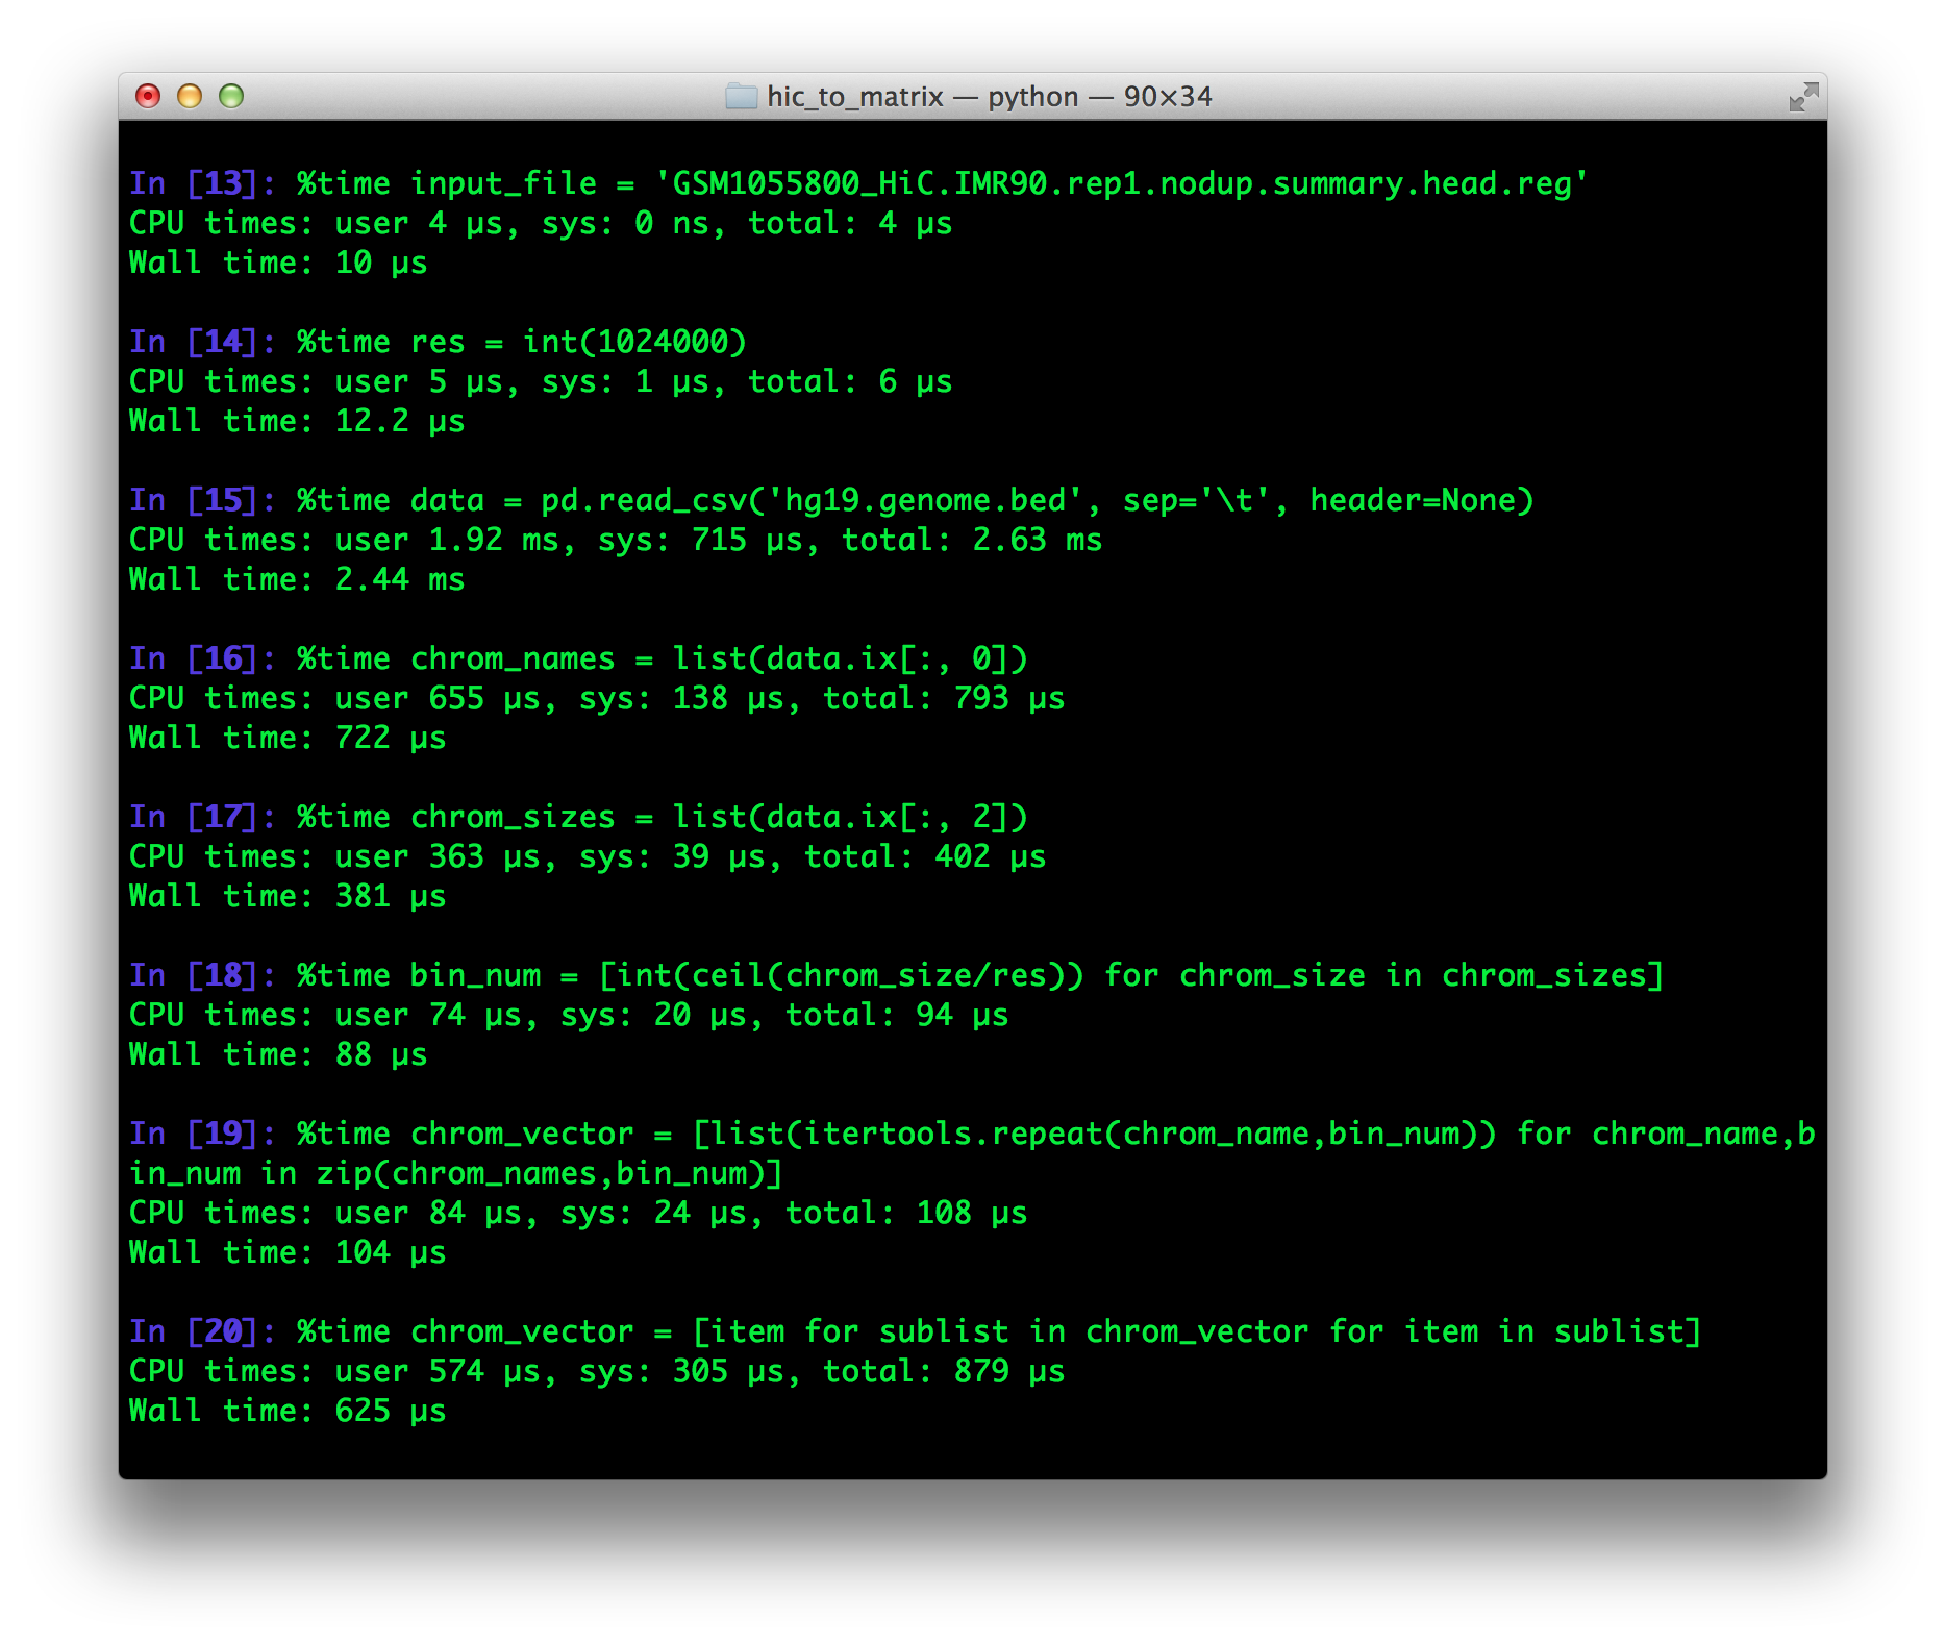
\includegraphics[max size={\textwidth}{\textheight}]{./Figures-Timing/first_program_part.pdf}
	\end{center}
	\caption{Time taken to run the first part}
	\label{fig:figure3}
\end{figure}

\begin{figure}[!htb]
	\begin{center}
		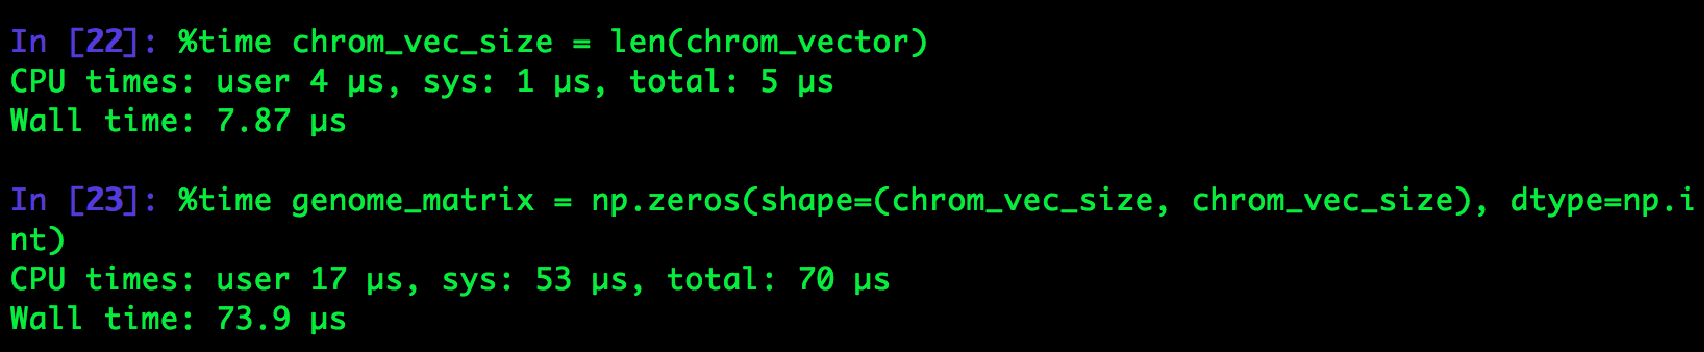
\includegraphics[max size={\textwidth}{\textheight}]{./Figures-Timing/second_program_part.pdf}
	\end{center}
	\caption{Time taken to run the second part}
	\label{fig:figure4}
\end{figure}

Below, I present the most time-consuming parts that consist of
reading and writing files:

\begin{figure}[!htb]
	\begin{center}
		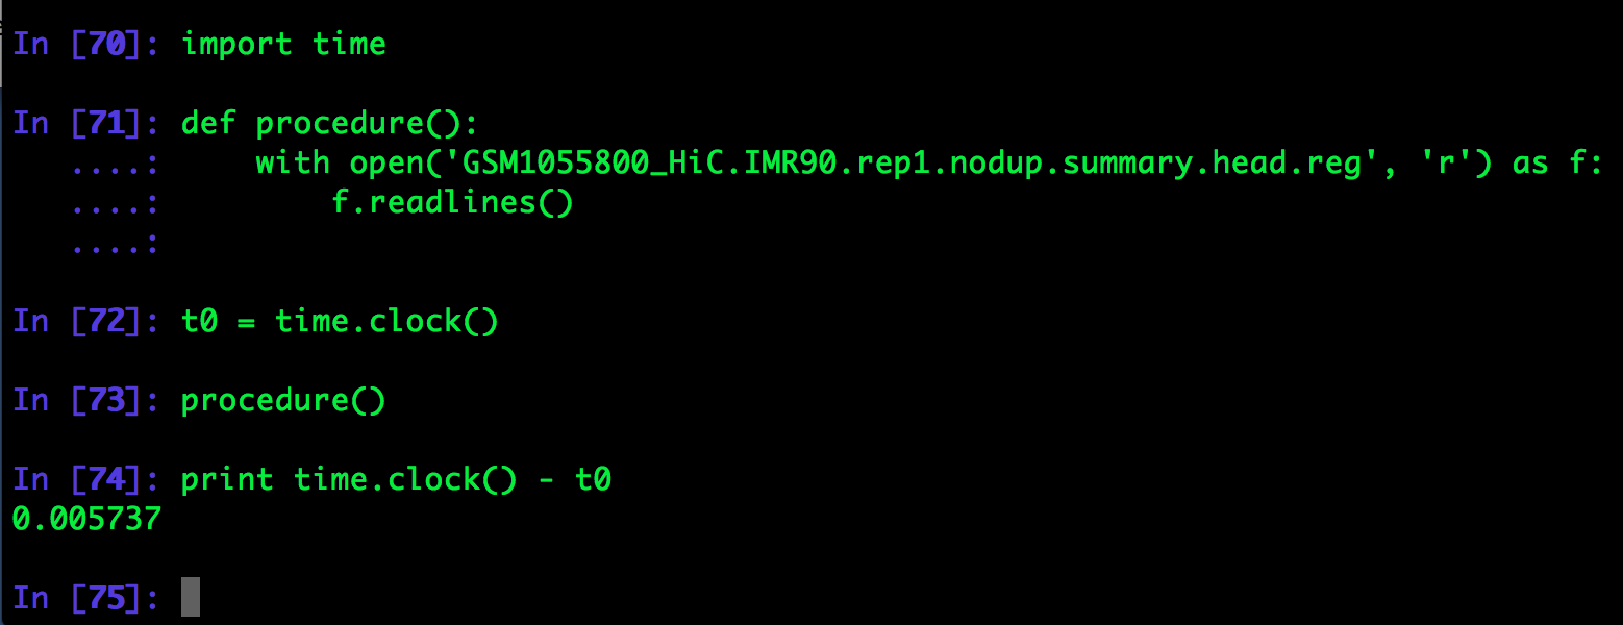
\includegraphics[max size={\textwidth}{\textheight}]{./Figures-Timing/time_to_read_file_in_sec.pdf}
	\end{center}
	\caption{Time taken to read input file}
	\label{fig:figure1}
\end{figure}

\begin{figure}[!htb]
	\begin{center}
		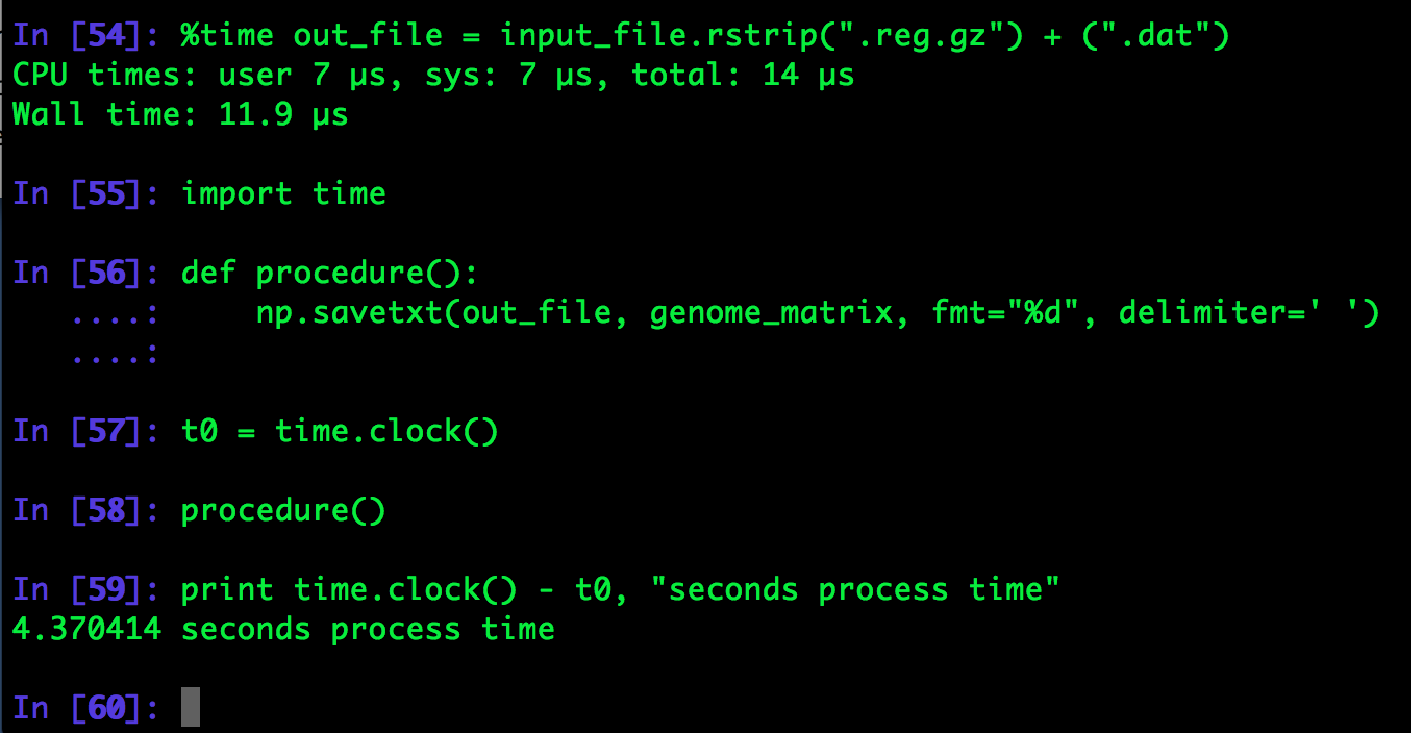
\includegraphics[max size={\textwidth}{\textheight}]{./Figures-Timing/writing_the_matrix_takes_time.pdf}
	\end{center}
	\caption{Time taken to write the output file}
	\label{fig:figure1}
\end{figure}


\subsection*{Focus area}

I focused on the use of Python packages (Numpy, Pandas)
as well as on visualization (with matplotlib and Pandas). 
R was used for the creation of heatmaps.

In Figure ~\ref{fig:figure1} a heatmap of the murine chromosome
1 (genome version mm10), is presented. The resolution is 1MB 
and in the case of the left panel, HindIII was used for the Hi--C
experiment, while for Figure~\ref{fig:figure1}, NcoI was used to perform Hi--C.

While it is obvious that the intra-chromosomal interactions (represented by the main diagonal) are much more frequent that the
inter-chromosomal ones in both A and B, there are clearly differences between the two heatmaps.

\begin{figure}[!htb]
	\begin{center}
		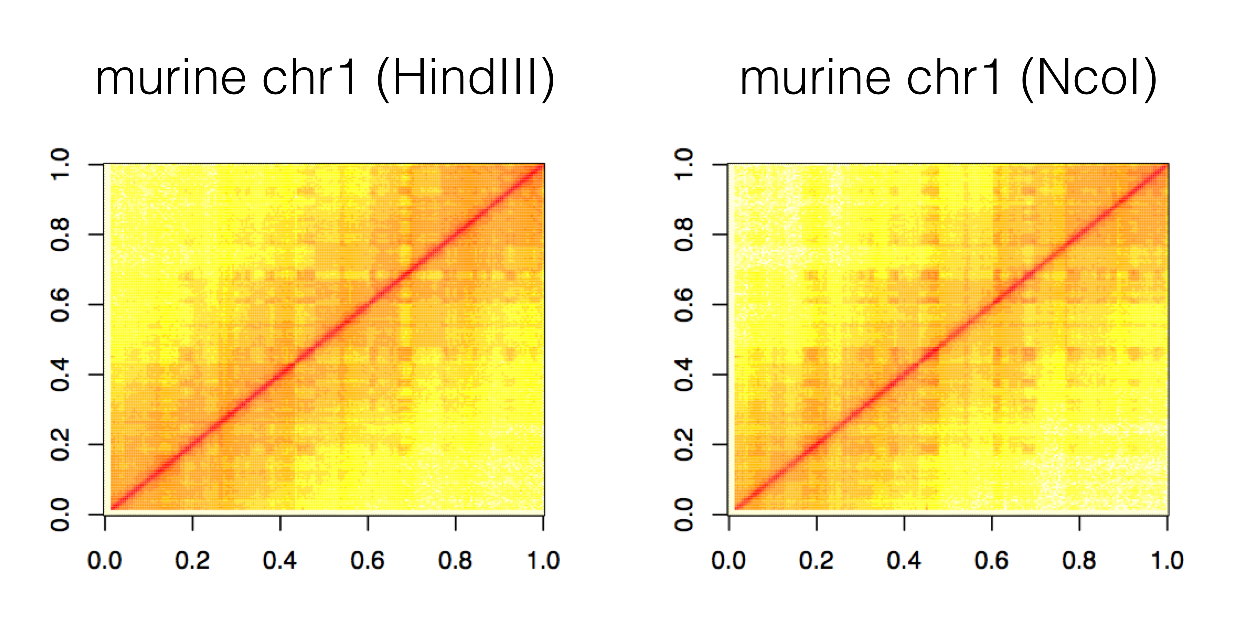
\includegraphics[max size={\textwidth}{\textheight}]{./Figures/murine_HindIII_NcoI.pdf}
	\end{center}
	\caption{Heatmaps showing intrachromosomal (\emph{cis}) and
	interchromosomal (\emph{trans}) interactions in the case of murine chromosome 1. The Hi--C experiment was performed using 
	HindIII in A and NcoI in B}.
	\label{fig:figure1}
\end{figure}

After finding this difference between the contact matrices generated by the two different enzymes, I went on analysing the correlation of the contact matrices of all 23 chromosomes (22 autosomes \& X) for different resolutions (128kb, 1024kb, 4096kb) and for all possible combinations of restriction enzymes.

In the case of 128kb (Figure ~\ref{fig:figure2}), the correlation values were the smallest ones. Moreover, it appears that the normalization method (HiCNorm)
used was not particularly good as it may increase the correlation
when different enzymes were used but it decreased it in the case
of the same enzyme (which should not be the case).

\begin{figure}[!htb]
	\begin{center}
		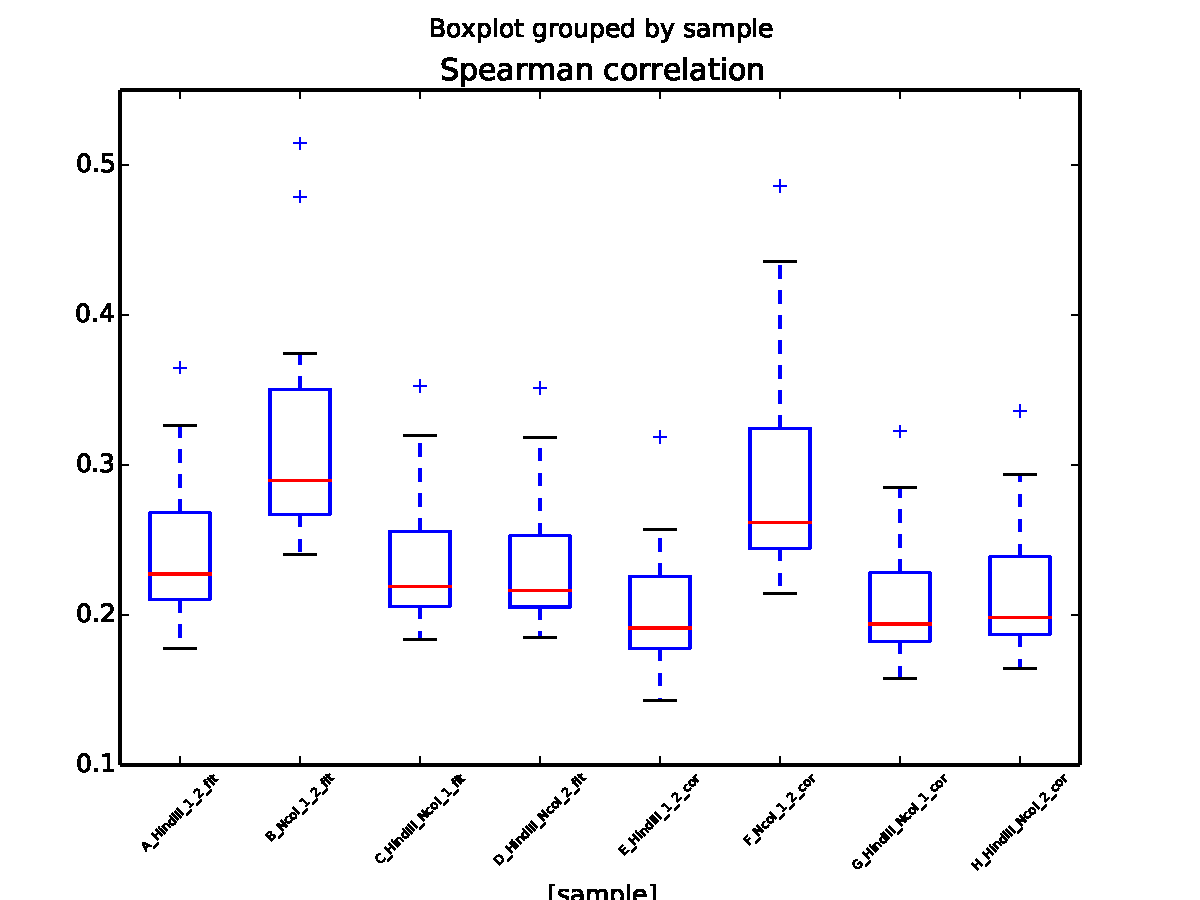
\includegraphics[max size={\textwidth}{\textheight}]{./Figures/128_boxplot.pdf}
	\end{center}
	\caption{Boxplots showing Spearman correlation for all chromosomes and across different samples (HindIII vs HindIII filtered, NcoI vs NcoI filtered, HindIII vs NcoI replicate I filtered, HindIII vs NcoI replicate 2 filtered, HindIII vs HindIII corrected, NcoI vs NcoI corrected, HindIII vs NcoI replicate I corrected, HindIII vs NcoI replicate 2 corrected). Resolution 128kb}.
	\label{fig:figure2}
\end{figure}

In the case of 1024kb resolution (Figure~\ref{fig:figure3}), the correlation is increased but when the same enzyme is used, the correction does not perform well (simply filtered samples appear to be more highly correlated than the corrected ones).

\begin{figure}[!htb]
	\begin{center}
		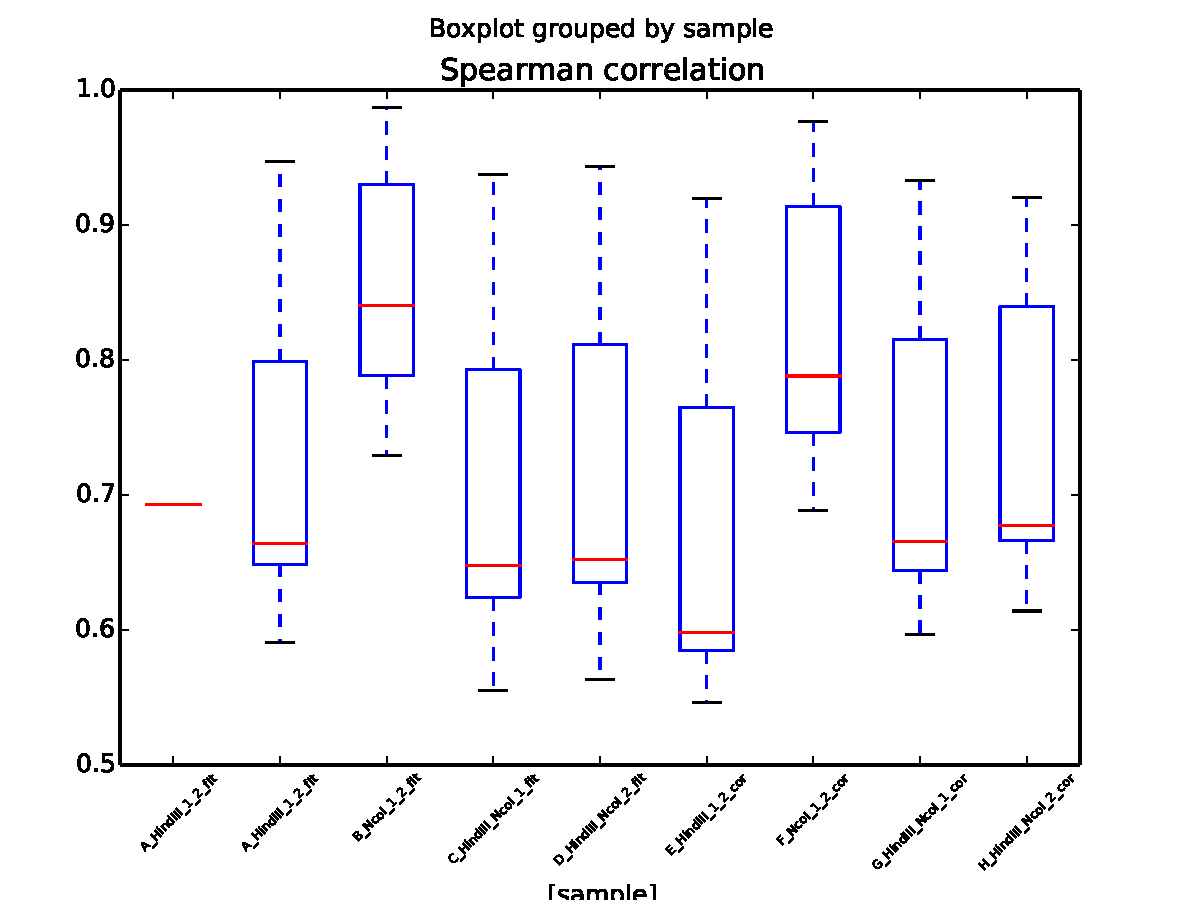
\includegraphics[max size={\textwidth}{\textheight}]{./Figures/1024_boxplot.pdf}
	\end{center}
	\caption{Boxplots showing Spearman correlation for all chromosomes and across different samples (HindIII vs HindIII filtered, NcoI vs NcoI filtered, HindIII vs NcoI replicate I filtered, HindIII vs NcoI replicate 2 filtered, HindIII vs HindIII corrected, NcoI vs NcoI corrected, HindIII vs NcoI replicate I corrected, HindIII vs NcoI replicate 2 corrected). Resolution 1024kb}.
	\label{fig:figure3}
\end{figure}

Finally, as the resolution becomes even more coarse, the correlation increases even further (Figure~\ref{fig:figure4}).

\begin{figure}[!htb]
	\begin{center}
		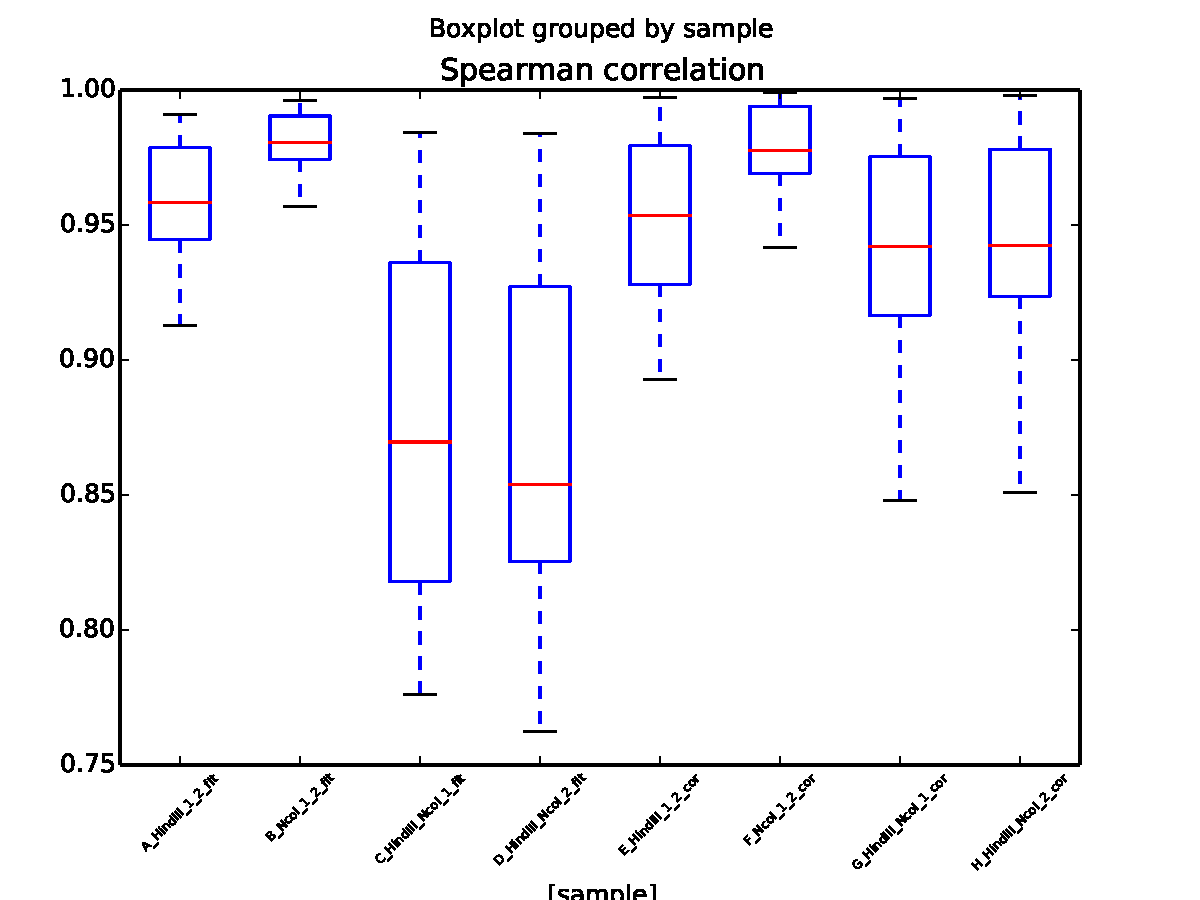
\includegraphics[max size={\textwidth}{\textheight}]{./Figures/4096_boxplot.pdf}
	\end{center}
	\caption{Boxplots showing Spearman correlation for all chromosomes and across different samples (HindIII vs HindIII filtered, NcoI vs NcoI filtered, HindIII vs NcoI replicate I filtered, HindIII vs NcoI replicate 2 filtered, HindIII vs HindIII corrected, NcoI vs NcoI corrected, HindIII vs NcoI replicate I corrected, HindIII vs NcoI replicate 2 corrected). Resolution 4096kb}.
	\label{fig:figure4}
\end{figure}



% \begin{wrapfigure}{l}{0.4\textwidth} % Inline image example
% \begin{center}
% \includegraphics[width=0.018\textwidth]{fish.png}
% \end{center}
% \caption{Fish}
% \end{wrapfigure}


%------------------------------------------------

\section*{Conclusion-Discussion}

It is clear from the analysis presented in this study that
even state-of-the-art Hi--C analysis techniques do not
give extremely reproducible results. When two different
restriction enzymes are used with the same sample as source,
while the correlation is relatively high, it is not ideal.
Moreover, when the resolution is increased (128kb bins instead
of 4096kb bins), the correlation even in the case of technical
replicates treated with the same enzymes is very low. Thus, new
more robust analysis techniques that lead to more reproducible
results, are required. This is going to be a large part of my 
PhD thesis work.

While I optimized the code for speed, by using Numpy instead of
native Python to deal with matrices and list comprehension insted
of for loops when possible, the real bottleneck is the I/O operations
(reading input and writing output). This is critical as the matrix
files that I have to deal with, are really large. One solution to
the problem would be to minimize I/O operations by using Numpy
for everything, but this would require much better knowledge
of Numpy than I currently have. Moreover, Numpy may be not as versatile
or efficient as R in certain circumstances which means that 
I may be unable to fully replace R with Numpy. Another approach 
would be to use rpy or rpy2 for R/Python integration but I have been
always facing problems with rpy/rpy2 installation on my system.

As far as the visualization is concerned, both Pandas and matplotlib
look interesting but:

\begin{enumerate}
\item They need time to learn.  
\item There are many requirements (dependencies etc) and in many
cases it is difficult to run code using these packages on the cluster.
\item The resulting graphs, especially in the case of Pandas, do not
seem to be extremely customizable. Moreover, I had to write more
code to achieve the same result I would get with writing less
code in R.
\end{enumerate}

I will certainly try to explore Numpy, matplotlib, Pandas and other
packages further, as it is always possible that the drawbacks I see
right now compared to R may be just due to luck of expertise on all
these Python packages. 

%-------------------------------------------------------------------------------------
%	BIBLIOGRAPHY
%-------------------------------------------------------------------------------------

\bibliographystyle{unsrt}

\bibliography{Hi-C}

%-------------------------------------------------------------------------------------

\end{document}